\documentclass[10pt, aspectratio=169]{beamer}
\usetheme{metropolis}

\usepackage{appendixnumberbeamer}
\usepackage{booktabs}
\usepackage[scale=2]{ccicons}
\usepackage{pgfplots}
\usepgfplotslibrary{dateplot}
\usepackage{xspace}
\usepackage{helvet}
\usepackage{multimedia}

% Change Color of the theme
\usepackage{xcolor}
\definecolor{backgrnd}{HTML}{FFFFFF}
\definecolor{text}{HTML}{111116}
\definecolor{accent}{HTML}{d5697d}
\setbeamercolor{normal text}{ fg= text, bg= backgrnd  }
\setbeamercolor{alerted text}{ fg= accent  }
\setbeamercolor{background canvas}{bg= backgrnd }

% Change item spacing of itemize
\newenvironment{items}{
    \begin{itemize}
    \setlength{\itemsep}{10pt}
    \setlength{\parskip}{0pt}
    \setlength{\parsep}{0pt}}{
\end{itemize}
}

%%%%%%%%%%%%%%%%%%%%%%%%%%%%%%%%%%%%%%%%%%%%%%%%%%%%%%%%%%%%%%%%%%%%%%%%%%%%%%%

\title{My personal slide templates using the amazing \\minimalistic beamer tempate \texttt{metropolis}}
\subtitle{A nice subtitle}
\author{Patrick Weygoldt}
% \institute{Neuroethology Group, University of Tuebingen}
\date{}
% \titlegraphic{\hfill\includegraphics[height=1.5cm]{logo.pdf}}

%%%%%%%%%%%%%%%%%%%%%%%%%%%%%%%%%%%%%%%%%%%%%%%%%%%%%%%%%%%%%%%%%%%%%%%%%%%%%%%

\begin{document}

\begin{frame}[standout]{}
\end{frame}

% a slide with a full screen video
% a tikzpicture is used to make the video fullscreen, without
% trial and error
\begin{frame}[standout]{}
    \begin{tikzpicture}[remember picture,overlay]
        \node[at=(current page.center)] {
        \movie[
            autostart, % play automatically
            repeat, % repeat the movie
            poster, % show the first frame
            loop, % loop the movie
            width=\paperwidth,
            height=\paperheight]{}{assets/movie.mp4}};
    \end{tikzpicture}
\end{frame}

\maketitle

\section{Communication}

\begin{frame}[fragile]{Electrocommunication}
    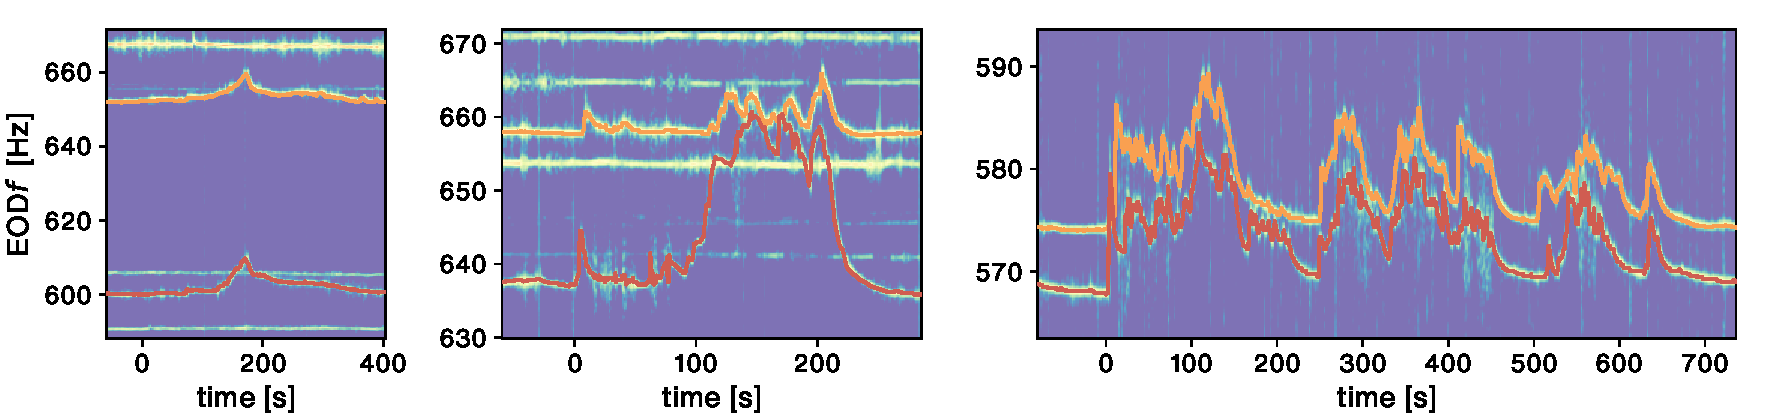
\includegraphics[width=\textwidth]{assets/selected_modulations.pdf}
\end{frame}

\begin{frame}[fragile]{Electrocommunication}
    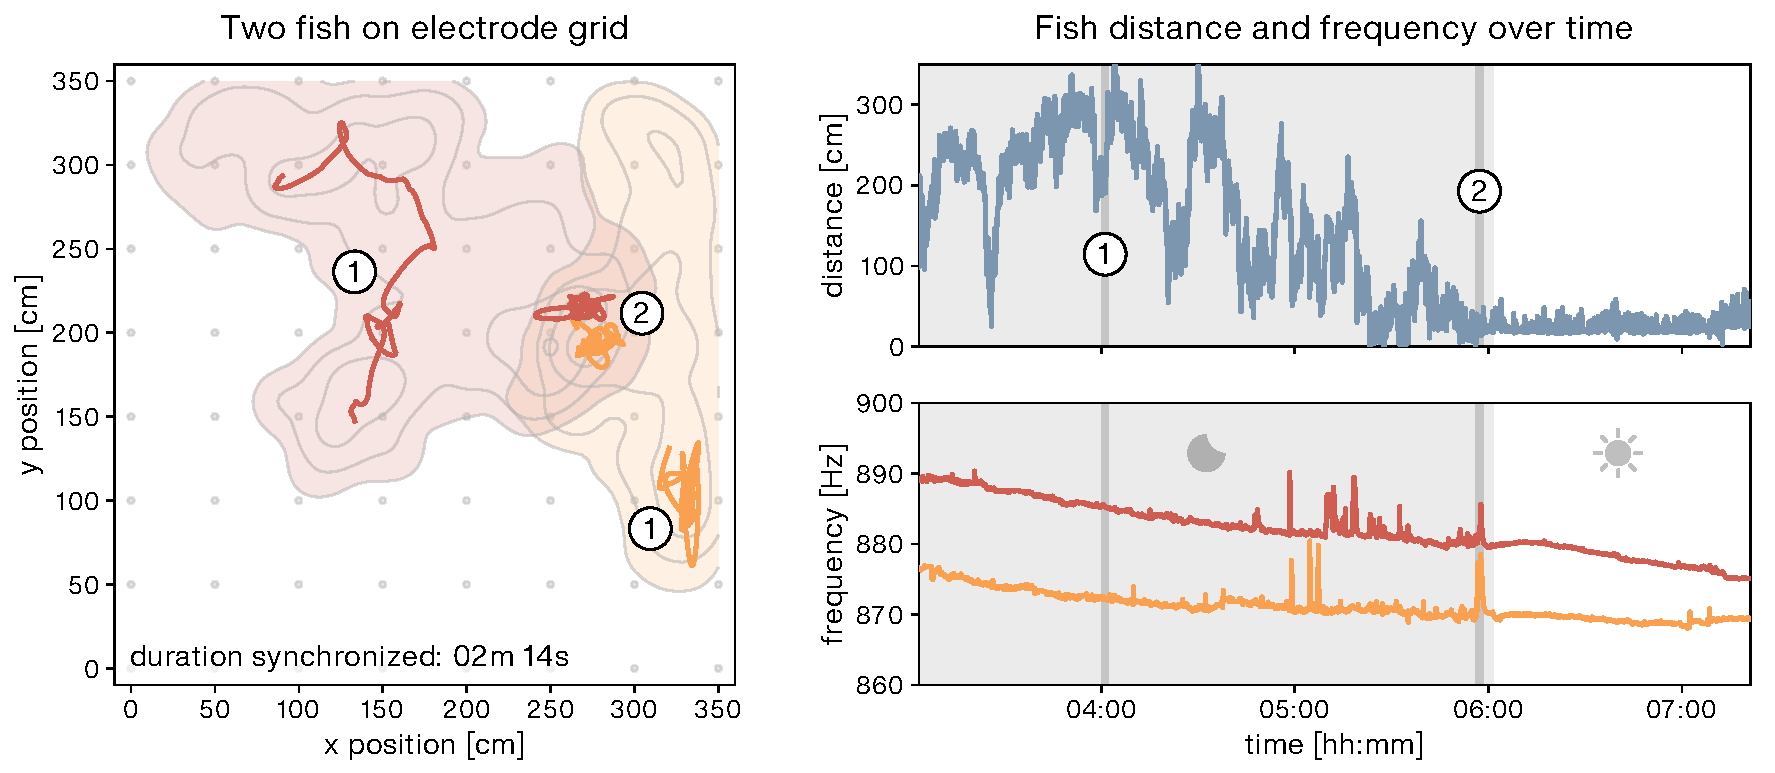
\includegraphics[width=\textwidth]{assets/eventposition_2.pdf}
\end{frame}

\begin{frame}[fragile]{Electrocommunication}
    \begin{minipage}[c]{0.5\textwidth}
    \begin{items}
        \item This is the first item of the list.
        \item This item is a little bit longer than\\the first one, to  show
            how the \\spacing looks like.
        \item This item is shorter.
    \end{items}
    \end{minipage}%
    \begin{minipage}[c]{0.5\textwidth}
        \vspace{0.5cm}
        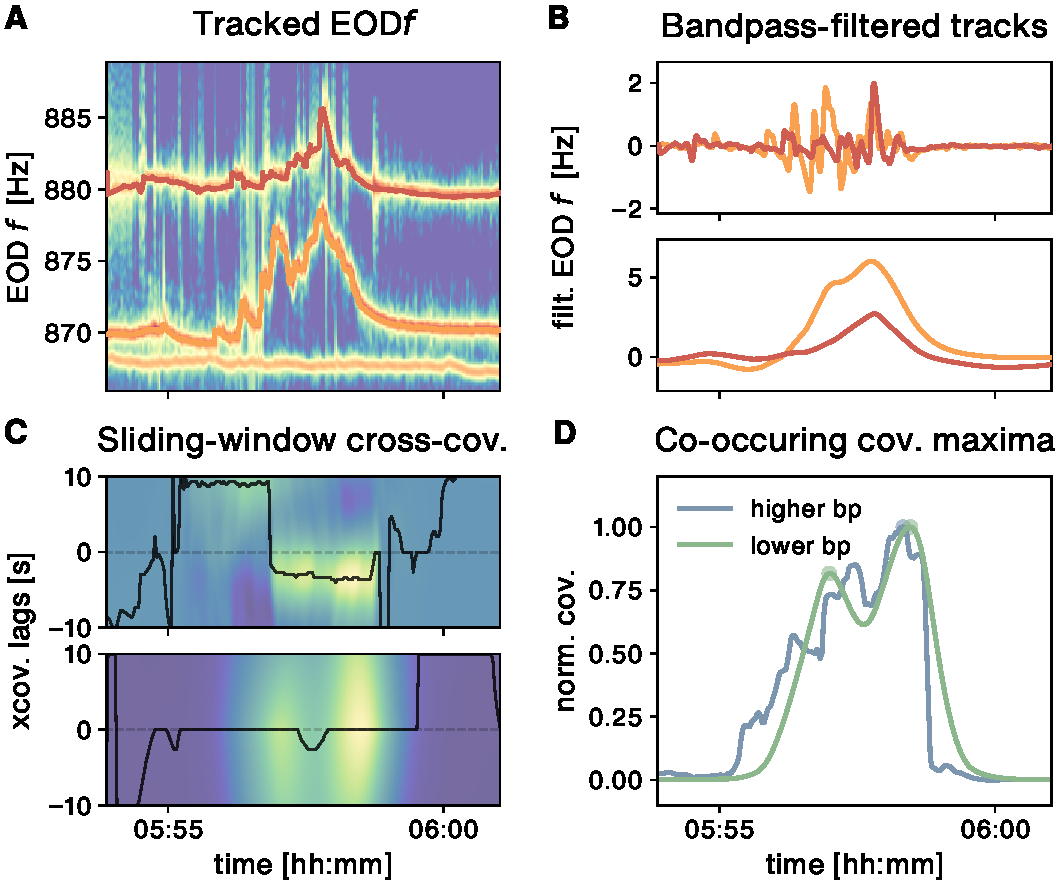
\includegraphics[width=\textwidth]{
            assets/CovDetector_backend_ids_26788_26789_index_0.pdf}
    \end{minipage}%
\end{frame}

\begin{frame}[standout]
    This is \alert{important} information\\
    that has to be \alert{highlighted}.
\end{frame}

\section{Spatiotemporal behaviours}

\begin{frame}[fragile]{Spatiotemporal behaviours}
    \begin{minipage}[c]{0.5\textwidth}
    \begin{items}
        \item This is the first item of the list.
        \item This item is a little bit longer than\\the first one.
        \item This item is shorter.
    \end{items}
    \end{minipage}%
    \begin{minipage}[c]{0.5\textwidth}
        \movie[
            repeat, % repeat the movie
            poster, % show the first frame
            loop, % loop the movie
            width=\linewidth,
            height=0.5\paperheight
            ]{}{assets/movie.mp4}
    \end{minipage}%
\end{frame}

\begin{frame}[standout]
    Thank you!
\end{frame}

\appendix % all slides after this will not be numbered

\begin{frame}[fragile]{Appendix}
    \begin{minipage}[c]{0.5\textwidth}
    \begin{items}
        \item This is the first item of the list.
        \item This item is a little bit longer than\\the first one.
        \item This item is shorter.
    \end{items}
    \end{minipage}%
    \begin{minipage}[c]{0.5\textwidth}
        \vspace{0.5cm}
        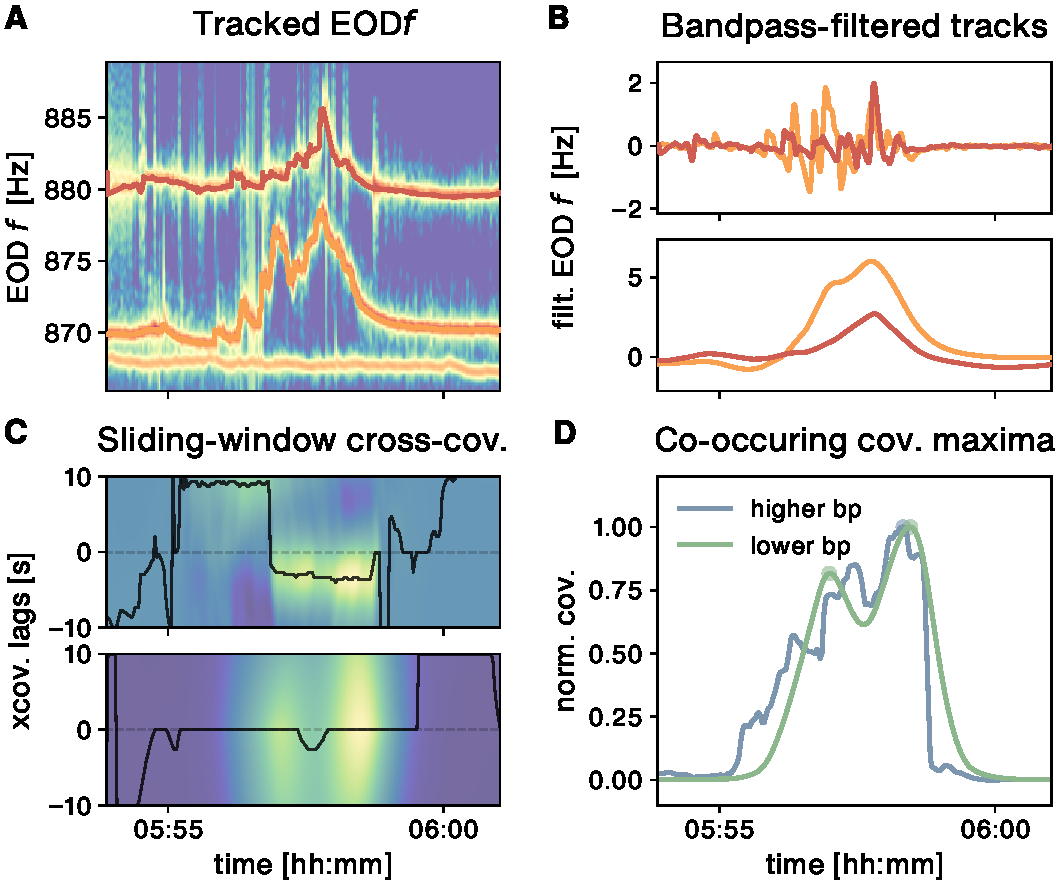
\includegraphics[width=\textwidth]{
            assets/CovDetector_backend_ids_26788_26789_index_0.pdf}
    \end{minipage}%
\end{frame}

\begin{frame}[standout]
$$\sigma_x^2 =
\frac{1}{2\pi}\int_{-\infty}^{\infty}X^*(\omega)\underbrace{\int_{-\infty}^{\infty} X(\nu) \underbrace{\frac{1}{2\pi}\int_{-\infty}^{\infty} e^{-i(\omega-\nu)t}\; dt}_{\delta(\omega-\nu)} \; d\nu}_{X(\omega)} \; d \omega
$$
\end{frame}

\end{document}
